В отличие от классического подхода, в котором
параметрические модели $f(x,\theta)$, не имеют заданного
вероятностного распределения байесов вывод
требует задания априорного распределения на $\theta$ :
\begin{equation}
    P(\theta | X) = \frac{P(X| \theta|) P(\theta)}{P(X)}
\end{equation}

В современной литературе 
исследователи обращают особенное внимание 
на маргинальное распределение $P(X) = \int P(X, \theta) d\theta$
В теории причинно-следственного анализа введенную величину
свидетельство. (\texit{англ.} Evidence). Максимизация свидетельства
позволяет выбирать модели согласно принципу бритву Оккама, исключать
параметры не вносящие существенного смысла для модели.

Для расчета свидетельства необходимо выполнить маргинализацию по параметрам
модели $\int P(X, \theta) d\theta$. В общем случае задача принадлежит 
NP-классу сложности, рассчитывается за время, экспоненциально зависящее
от числа параметров. Тем не менее классы моделей, представимых в виде
древа имеют линейную сложность. Для выделения 


\texit{Определение} События $A$ и $B$ cчитаются независимыми в условиях:
\begin{equation}
    P(A \cup B) = P(A) \times P(B)
\end{equation}

Многокомпонетный осложняется неоднозначной трактовкой исхода. 
Для анализа сложных систем предпочтителен однофакторный анализ, выполняющий
для его выполнения необходимо перекрыть потоки зависимостей (\textit{англ.} dependecy flow) от
прочих переменных.


\texit{Определение} События $A$ и $B$ cчитаются независимыми в условиях:
\begin{equation}
    P(A \cup B) = P(A) \times P(B)
\end{equation}

На практике в системах подлинная независимость случайных величин $x$ и $y$
$x \perp y$ встречается не всегда. 
Чаще достижима условная независимость, наблюдаемая при
фиксации третьего фактора $z$.

\texit{Определение} События $A$ и $B$ cчитаются условно независимыми 
для заданного события $C$ в условиях:
\begin{equation}
    P(A \cup B |C) = P(A|C) \times P(B|C)
\end{equation}

Условная независимость позволяет 
$x \perp y$ встречается не всегда.

\texit{Определение} \texbf{Алгоритм исключения переменных}

\texit{Определение} \textbf{Байесовой сетью} называется направленный граф $G=(V,E)$ такой, что  
$\forall V \rightarrow x_i \sim p(x_i| x_{A_i})$, где $x_{A_i}$ - родительские злы 

\begin{figure}[h]
    \centering
    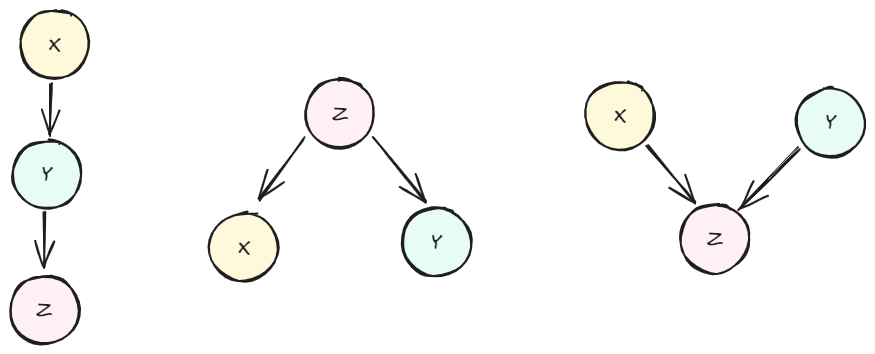
\includegraphics[width=0.5\textwidth]{assets/math/discrete/bayes_net.excalidraw.png}
    \caption{Посредник(\textit{англ.} mediator), общий предок(\textit{англ.} cofounder), 
 общий родственник \textit{англ.} collider) }
    \label{discr_vs_gen}
\end{figure}


Расчет маргинального распределения

\begin{figure}[h]
    \centering
    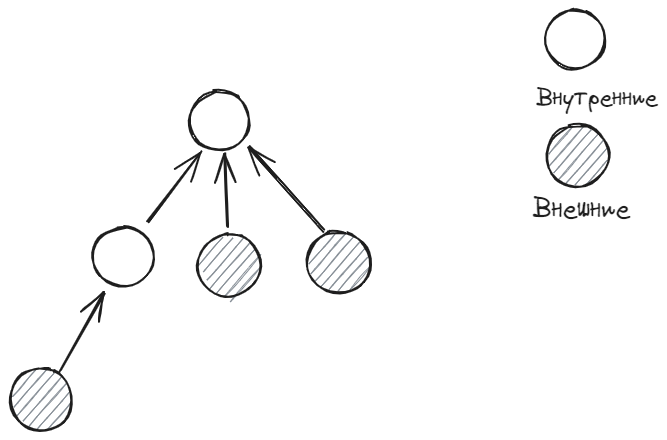
\includegraphics[width=0.5\textwidth]{assets/math/discrete/belief_propogation.excalidraw.png}
    \caption{H}
    \label{discr_vs_gen}
\end{figure}

Отбор оптимальной графической модели выполняется 
исходя из максимизации доказательства (\texit{англ.} Evidence)
\begin{equation}
    P(E) = 
\end{equation}




\begin{figure}[h]
    \centering
    
\includegraphics[width=0.5\textwidth]{assets/math/discrete/junction_tree.excalidraw.png}
    \caption{H}
    \label{discr_vs_gen}
\end{figure}


\textit{Определение} \textbf{Марковские случайные поля} это
вероятностное распределение $p$, заданное на переменных $x_1, \dots,x_n$, образующих
граф $G=(V,E)$, для которого выполняется \begin{itemize}
    \item 
    \item  совместное распределение $p(\mathbf{x})$ задается через  \begin{equation}
        p(x_1, \dots, x_n) = \frac{1}{Z} \prod_{c \in C} \phi_c(x_c),
    \end{equation} где $Z = \sum_{x_1, \dots}$ - нормализующая переменная.
\end{itemize}

\textit{Определение} \textbf{Марковским покрытие} (\texit{англ.} Markov blanket)  $U$ переменной X 
в графе $G$ называется минимальной число узлов, таких что $X$   
это
 
Одним из распространенных представлений марковских полей
является фактор граф \ref{}





